% ============================================================================
%  Informe Técnico — OmniRec-Movies / OmniCine
%  Sistema Inteligente de Recomendación de Películas (MovieLens 25M)
%  Documenta: catálogo de modelos, arquitectura general, MLOps y web-app.
%
%  Compilar:  pdflatex Informe_Tecnico_OmniRec.tex   (x2 para el índice)
%  Requiere paquetes estándar de TeXLive (tcolorbox, titlesec, tikz, listings).
% ============================================================================
\documentclass[11pt,a4paper]{article}

% ------------------------------------------------------------------ idioma/fuentes
\usepackage[utf8]{inputenc}
\usepackage[T1]{fontenc}
\usepackage[spanish,es-noshorthands]{babel}
\usepackage{lmodern}
\usepackage{microtype}

% ------------------------------------------------------------------ layout
\usepackage[a4paper,margin=2.4cm,headheight=15pt]{geometry}
\usepackage{graphicx}
\graphicspath{{figures/}}
\usepackage{booktabs}
\usepackage{tabularx}
\usepackage{array}
\usepackage{longtable}
\usepackage{enumitem}
\setlist{nosep,leftmargin=1.4em}
\usepackage{titlesec}
\usepackage{fancyhdr}
\usepackage[most]{tcolorbox}
\usepackage{listings}
\usepackage{tikz}
\usetikzlibrary{shapes.geometric,arrows.meta,positioning,calc,fit,backgrounds}

% ------------------------------------------------------------------ paleta
\definecolor{omniprimary}{HTML}{0B3D5C} % azul profundo
\definecolor{omniaccent}{HTML}{1B998B}  % verde azulado
\definecolor{omnidark}{HTML}{12233A}
\definecolor{omnilight}{HTML}{EEF3F6}
\definecolor{omnisoft}{HTML}{DCE7EC}
\definecolor{omnigray}{HTML}{5B6770}
\definecolor{omnigold}{HTML}{C9A227}
\definecolor{codebg}{HTML}{F4F6F8}

% ------------------------------------------------------------------ hyperref
\usepackage[colorlinks=true,linkcolor=omniprimary,urlcolor=omniaccent,citecolor=omniaccent]{hyperref}

% ------------------------------------------------------------------ títulos
\titleformat{\section}
  {\color{omniprimary}\Large\bfseries\sffamily}
  {\color{omniaccent}\thesection}{0.8em}{}[{\color{omnisoft}\titlerule[1.2pt]}]
\titleformat{\subsection}
  {\color{omnidark}\large\bfseries\sffamily}
  {\color{omniaccent}\thesubsection}{0.7em}{}
\titleformat{\subsubsection}
  {\color{omnidark}\normalsize\bfseries\sffamily}
  {}{0em}{}
\titlespacing*{\section}{0pt}{16pt}{8pt}

% ------------------------------------------------------------------ encabezado/pie
\pagestyle{fancy}
\fancyhf{}
\renewcommand{\headrulewidth}{0.4pt}
\renewcommand{\footrulewidth}{0pt}
\fancyhead[L]{\footnotesize\sffamily\color{omnigray}OmniRec-Movies}
\fancyhead[R]{\footnotesize\sffamily\color{omnigray}Informe Técnico}
\fancyfoot[C]{\thepage}

% ------------------------------------------------------------------ código
\lstdefinestyle{omni}{
  backgroundcolor=\color{codebg},
  basicstyle=\ttfamily\footnotesize\color{omnidark},
  keywordstyle=\color{omniprimary}\bfseries,
  commentstyle=\color{omnigray}\itshape,
  stringstyle=\color{omniaccent},
  numbers=none, frame=single, rulecolor=\color{omnisoft},
  framesep=6pt, xleftmargin=8pt, breaklines=true, showstringspaces=false,
  literate={á}{{\'a}}1 {é}{{\'e}}1 {í}{{\'i}}1 {ó}{{\'o}}1 {ú}{{\'u}}1 {ñ}{{\~n}}1 {Á}{{\'A}}1 {→}{{$\rightarrow$}}1 {·}{{\textperiodcentered}}1 {—}{{---}}1 {–}{{--}}1
}
\lstset{style=omni}
\newcommand{\code}[1]{\textcolor{omnidark}{\texttt{#1}}}

% ------------------------------------------------------------------ caja "ficha de modelo"
\newtcolorbox{modelcard}[2][]{
  enhanced, breakable, colback=omnilight, colframe=omniprimary,
  boxrule=0.8pt, arc=3pt, left=10pt, right=10pt, top=8pt, bottom=8pt,
  fonttitle=\bfseries\sffamily, coltitle=white, colbacktitle=omniprimary,
  title={#2}, #1
}
\newtcolorbox{infobox}[1][Nota]{
  enhanced, breakable, colback=omnisoft!40, colframe=omniaccent,
  boxrule=0.8pt, arc=2pt, left=8pt, right=8pt, top=6pt, bottom=6pt,
  fonttitle=\bfseries\sffamily, coltitle=white, colbacktitle=omniaccent, title={#1}
}
% etiquetas de estado
\newcommand{\enprod}{\textcolor{white}{\colorbox{omniaccent}{\scriptsize\bfseries\,EN PRODUCCIÓN\,}}}
\newcommand{\noserv}{\textcolor{white}{\colorbox{omnigray}{\scriptsize\bfseries\,SOLO DOCUMENTACIÓN\,}}}
\newcommand{\proceso}{\textcolor{white}{\colorbox{omnigold}{\scriptsize\bfseries\,PROCESO / SELECCIÓN\,}}}

\newcolumntype{L}[1]{>{\raggedright\arraybackslash}p{#1}}

% ============================================================================
\begin{document}
\sffamily

% ------------------------------------------------------------------ PORTADA
\begin{titlepage}
\thispagestyle{empty}
\begin{tikzpicture}[remember picture,overlay]
  \fill[omniprimary] (current page.north west) rectangle ([yshift=-7.2cm]current page.north east);
  \fill[omniaccent]  ([yshift=-7.2cm]current page.north west) rectangle ([yshift=-7.6cm]current page.north east);
\end{tikzpicture}
\vspace*{0.6cm}
\begin{flushleft}
{\color{white}\fontsize{13}{16}\selectfont \textbf{UNIVERSIDAD CATÓLICA BOLIVIANA} \\[2pt]
\normalsize Machine Learning · Grupo 3}\\[1.6cm]
{\color{white}\fontsize{30}{34}\selectfont\bfseries OmniRec-Movies}\\[6pt]
{\color{omnisoft}\Large Sistema Inteligente de Recomendación\\[2pt] de Películas — \textit{OmniCine}}\\[3.0cm]
\end{flushleft}

\vfill
\begin{tcolorbox}[colback=omnilight,colframe=omniprimary,boxrule=0.8pt,arc=3pt]
\begin{minipage}{0.62\textwidth}
\textbf{\color{omniprimary}Informe Técnico Integral}\\[2pt]
\small Catálogo de modelos, arquitectura general, MLOps y plataforma web. Documenta el qué, el porqué, el para qué y el dónde de cada componente, sobre el dataset \textbf{MovieLens 25M} y la metodología \textbf{CRISP-DM}.
\end{minipage}\hfill
\begin{minipage}{0.32\textwidth}
\footnotesize
\textbf{Dataset:} MovieLens 25M\\
\textbf{Stack:} PyTorch · scikit-surprise · FAISS · FastAPI · Next.js 16\\
\textbf{MLOps:} pipeline + MLflow + Registry + Monitoreo\\
\textbf{Fecha:} 24 de junio de 2026
\end{minipage}
\end{tcolorbox}
\end{titlepage}

% ------------------------------------------------------------------ RESUMEN + TOC
\pagenumbering{roman}
\section*{\color{omniprimary}Resumen ejecutivo}
\addcontentsline{toc}{section}{Resumen ejecutivo}
OmniRec-Movies es un sistema de recomendación de películas construido siguiendo el ciclo \textbf{CRISP-DM} de extremo a extremo: desde el entendimiento del negocio y el análisis exploratorio, pasando por el modelado clásico y profundo, hasta el despliegue como una plataforma web (\textit{OmniCine}) con una capa de \textbf{MLOps} reproducible. El proyecto combina \textbf{tres familias de modelos} que se reparten el trabajo según el contexto: factorización matricial clásica (\textbf{SVD}) para la recomendación personalizada, redes neuronales de embeddings (\textbf{MF+Bias / NeuMF}) para la similitud entre películas, y recuperación semántica con \textit{transformers} (\textbf{MiniLM + FAISS + LLM}) para la búsqueda en lenguaje natural. Todos los modelos servidos están \textbf{versionados} con manifiestos SHA256, \textbf{trackeados} en MLflow y \textbf{monitoreados} frente a \textit{drift} y degradación. Este informe documenta cada modelo en detalle, la arquitectura global, el funcionamiento de la capa MLOps y cómo cada pieza se traduce en una funcionalidad concreta de la web-app.

\vspace{6pt}
\begin{infobox}[Cómo leer este documento]
La Sección~\ref{sec:arq} ofrece el \textbf{panorama general}. La Sección~\ref{sec:modelos} es el \textbf{catálogo detallado de modelos} (una ficha por modelo). La Sección~\ref{sec:produccion} resume \textbf{qué se usa en producción y dónde}. La Sección~\ref{sec:mlops} explica el \textbf{MLOps} en profundidad. La Sección~\ref{sec:webapp} describe la \textbf{web-app}.
\end{infobox}

\microtypesetup{protrusion=false}
\tableofcontents
\microtypesetup{protrusion=true}
\newpage
\pagenumbering{arabic}

% ============================================================================
\section{Introducción y panorama general}
\label{sec:intro}

\subsection{Objetivo del sistema}
El objetivo es recomendar películas relevantes a cada usuario y permitir descubrir contenido mediante búsqueda en lenguaje natural, sobre el catálogo de \textbf{MovieLens 25M} (25 millones de calificaciones, $\sim$62\,000 películas, 1\,128 \textit{tags} del \textit{Tag Genome}). El sistema atiende tanto a \textbf{usuarios registrados} (con historial) como a \textbf{invitados} (sin historial), por lo que la estrategia de modelado debe resolver explícitamente el problema de \textit{cold-start}.

\subsection{Metodología: CRISP-DM por fases}
El proyecto se organiza en \textit{notebooks} que corresponden a las fases de CRISP-DM, y en un código de producción (\code{src/}, \code{app/}) que materializa el despliegue y la operación.

\begin{center}
\small
\begin{tabularx}{\textwidth}{@{}l l X@{}}
\toprule
\textbf{Fase CRISP-DM} & \textbf{Notebook / Módulo} & \textbf{Aporte} \\
\midrule
1. Business + Data Understanding & \code{01\_Business\_Understanding\_and\_EDA} & Análisis exploratorio, comprensión del dominio. \\
2. Data Preparation & \code{02\_Data\_Sampling\_and\_Cleaning} & Muestreo estratificado, limpieza, \textit{parquets}. \\
3. Modeling (clásico) & \code{03\_ML\_Baseline\_AutoML} & Baseline, KNN, SVD, NMF, AutoML, KMeans. \\
4. Modeling (profundo) & \code{04\_DeepLearning\_Embeddings} & MF+Bias y NeuMF (PyTorch). \\
4. RAG / recuperación & \code{05\_Semantic\_Search\_RAG} & Encoder MiniLM, FAISS, capa generativa. \\
4/5/6. MLOps + Deployment & \code{src/}, \code{app/}, \code{docker} & Pipeline, MLflow, registry, monitoreo, API+web. \\
\bottomrule
\end{tabularx}
\end{center}

\subsection{Stack tecnológico}
\begin{itemize}
\item \textbf{Modelado:} scikit-surprise (SVD, KNN, NMF), scikit-learn (KMeans), \textbf{PyTorch 2.4} (MF+Bias, NeuMF), Sentence-Transformers + \textbf{FAISS} (recuperación), Anthropic Claude (capa generativa).
\item \textbf{MLOps:} pipeline propio en \code{src/}, \textbf{MLflow} (tracking), \textit{model registry} con manifiestos SHA256, monitoreo de \textit{drift}.
\item \textbf{Servicio:} \textbf{FastAPI} (backend, puerto 8000), \textbf{Next.js 16} (frontend \textit{OmniCine}, puerto 3000), \textbf{Docker Compose} (orquestación).
\end{itemize}

% ============================================================================
\section{Arquitectura general del sistema}
\label{sec:arq}

El sistema separa con claridad el \textbf{entrenamiento} (offline, reproducible) del \textbf{servicio} (online, de baja latencia). Los modelos se entrenan en notebooks o en el pipeline, se persisten como \textbf{artefactos versionados}, y el backend los carga para servir inferencia a la web-app.

\begin{figure}[h]
\centering
\begin{tikzpicture}[
  font=\sffamily\footnotesize,
  box/.style={rounded corners=3pt,draw=omniprimary,fill=omnilight,thick,align=center,minimum height=0.95cm,inner sep=5pt},
  art/.style={rounded corners=3pt,draw=omniaccent,fill=omnisoft!50,thick,align=center,minimum height=0.9cm,inner sep=5pt},
  serv/.style={rounded corners=3pt,draw=omnigold,fill=omnilight,thick,align=center,minimum height=0.9cm,inner sep=5pt},
  arr/.style={-{Stealth[length=2.4mm]},omnigray,thick}
]
% capa datos
\node[box] (data) {\textbf{Datos}\\MovieLens 25M\\\textit{parquets}};
% entrenamiento
\node[box,right=1.0cm of data] (nb) {\textbf{Entrenamiento}\\Notebooks 03/04/05\\Pipeline \code{src/}};
% artefactos
\node[art,right=1.0cm of nb] (reg) {\textbf{Artefactos + Registry}\\svd · baseline\\dl\_embeddings · rag\_index\\\scriptsize(SHA256 + \textit{current})};
% backend
\node[serv,right=1.0cm of reg] (back) {\textbf{Backend}\\FastAPI\\\code{engine} · \code{semantic}};
% frontend
\node[serv,below=0.9cm of back] (front) {\textbf{Web-app}\\Next.js \textit{OmniCine}};
% mlops lateral
\node[box,below=0.9cm of nb,fill=omnisoft!40] (mlops) {\textbf{MLOps}\\MLflow · Monitoreo\\\textit{drift} · \textit{retrain}};

\draw[arr] (data) -- (nb);
\draw[arr] (nb) -- (reg);
\draw[arr] (reg) -- (back);
\draw[arr] (back) -- (front);
\draw[arr] (nb) -- (mlops);
\draw[arr] (mlops.east) -- ([yshift=-2pt]reg.west|-mlops.east);
\draw[arr,dashed] (back.south) -- (front.north);
\end{tikzpicture}
\caption{Flujo extremo a extremo: los datos alimentan el entrenamiento (offline), que produce artefactos versionados en el \textit{registry}; el backend los sirve a la web-app. La capa MLOps acompaña todo el ciclo.}
\label{fig:arq}
\end{figure}

\subsection{Componentes principales}
\begin{itemize}
\item \textbf{Datos} (\code{data/}): \textit{parquets} intermedios generados por los notebooks 02/03. El dataset canónico de servicio es \code{ratings\_knn\_10pct.parquet} (2,47\,M de calificaciones).
\item \textbf{Entrenamiento} (\code{notebooks/}, \code{src/}): los notebooks documentan el modelado; el pipeline \code{src/pipeline.py} lo reproduce de forma operativa.
\item \textbf{Artefactos + Registry} (\code{models/}): pesos y factores serializados, versionados en \code{models/registry/} con manifiestos SHA256.
\item \textbf{Backend} (\code{app/backend/}): FastAPI. \code{ml/engine.py} sirve recomendación y similitud; \code{ml/semantic.py} sirve búsqueda semántica y RAG.
\item \textbf{Frontend} (\code{app/web-app/}): Next.js 16 \textit{OmniCine}, consume la API REST.
\item \textbf{MLOps} (\code{src/}, \code{config/}, \code{docker}): pipeline, MLflow, registry, monitoreo y despliegue reproducible.
\end{itemize}

% ============================================================================
\section{Datos y preparación}
\label{sec:datos}
El notebook 02 realiza un \textbf{muestreo estratificado de usuarios} para obtener subconjuntos manejables sin sesgar la distribución de actividad, y persiste \textit{parquets} con compresión \textit{snappy}:

\begin{center}
\small
\begin{tabularx}{\textwidth}{@{}l r X@{}}
\toprule
\textbf{Artefacto} & \textbf{Tamaño} & \textbf{Uso} \\
\midrule
\code{ratings\_knn\_10pct.parquet} & 2,47\,M filas & Dataset canónico de servicio (entrenamiento DL y SVD operativo). \\
\code{movies\_prepared\_60pct.parquet} & 55\,113 filas & Catálogo (\code{movieId}, \code{title}, \code{genres}). \\
\code{genome\_scores\_prepared\_60pct.parquet} & 15,58\,M filas & Relevancia \textit{tag}--película (descriptores RAG). \\
\code{genome\_tags.parquet} & 1\,128 filas & Diccionario de \textit{tags} del \textit{Tag Genome}. \\
\code{item\_clusters.parquet} / \code{user\_clusters.parquet} & --- & Clústeres y estadísticos por película/usuario. \\
\bottomrule
\end{tabularx}
\end{center}

\begin{infobox}[Contrato de datos y Docker]
La imagen Docker incluye solo los \textit{parquets} necesarios para servir (vía \code{.dockerignore}); por eso el dataset operativo es \code{ratings\_knn\_10pct.parquet} y no los \textit{samples} de exploración. El pipeline resuelve automáticamente el primer \textit{parquet} de \textit{ratings} disponible (\code{src/data.py:resolve\_ratings\_path}).
\end{infobox}

% ============================================================================
\section{Catálogo de modelos}
\label{sec:modelos}
Esta sección documenta \textbf{cada modelo} con una ficha uniforme: qué es, cómo funciona, por qué se eligió, para qué sirve y dónde se usa (en documentación/notebook y en la web-app). El estado se etiqueta como \enprod{}, \noserv{} o \proceso{}.

% --------------------------------------------------------- baseline
\subsection{Baseline de popularidad bayesiana}
\begin{modelcard}{Baseline — Bayesian Weighted Rating \hfill \enprod}
\textbf{Qué es.} Ranking no personalizado que pondera la media de una película con un \textit{prior} global, evitando que películas con pocos votos dominen.\\[3pt]
\textbf{Cómo funciona.} $\text{score} = \frac{n}{n+m}\,\bar{r} + \frac{m}{n+m}\,C$, donde $\bar{r}$ es la media de la película, $n$ su número de votos, $C$ la media global y $m$ un umbral (cuantil de votos).\\[3pt]
\textbf{Por qué.} Es robusto, interpretable y resuelve el \textit{cold-start} de usuario: cuando no hay historial, no hay nada que personalizar.\\[3pt]
\textbf{Para qué / Dónde.} \emph{Documentación:} notebook 03. \emph{Web-app:} recomendaciones para invitados y \textit{pool} de candidatos a re-rankear. \emph{Backend:} \code{engine.popular()}, artefacto \code{baseline\_scores.pkl}.\\[3pt]
\textbf{Métricas (test temporal, nb03).} RMSE 1,009 · MAE 0,792 (línea base a superar).
\end{modelcard}

% --------------------------------------------------------- KNN
\subsection{KNN-Baseline (filtrado colaborativo por vecindario)}
\begin{modelcard}{KNN-Baseline (item-based, Pearson + ALS) \hfill \noserv}
\textbf{Qué es.} Filtrado colaborativo basado en vecinos: predice el rating combinando ítems similares al objetivo, corrigiendo por sesgos con \textit{baselines} ALS.\\[3pt]
\textbf{Cómo funciona.} Similitud \textit{pearson\_baseline} entre películas (\code{user\_based=false}), $k=40$ vecinos, \textit{min support} 5.\\[3pt]
\textbf{Por qué (y por qué NO se sirve).} Es un competidor clásico fuerte, pero quedó por detrás del SVD en RMSE y es costoso en memoria/latencia; no se persistió para producción.\\[3pt]
\textbf{Para qué / Dónde.} \emph{Documentación:} notebook 03 (comparación). \emph{Web-app:} no se usa.\\[3pt]
\textbf{Métricas (test temporal, nb03).} RMSE 0,893 · MAE 0,669.
\end{modelcard}

% --------------------------------------------------------- SVD
\subsection{SVD — Factorización matricial (modelo campeón clásico)}
\begin{modelcard}{SVD (Matrix Factorization) \hfill \enprod}
\textbf{Qué es.} Factorización de la matriz usuario--ítem en factores latentes; predice $\hat{r}_{ui} = \mu + b_u + b_i + q_i^\top p_u$.\\[3pt]
\textbf{Cómo funciona.} 50 factores, 20 épocas, \code{lr=0.005}, \code{reg=0.02} (scikit-surprise). Para \textbf{usuarios nuevos} aplica \textit{folding-in}: estima $p_u$ resolviendo un \textit{ridge} sobre los factores de los ítems que el usuario calificó (\code{engine.\_fold\_in}).\\[3pt]
\textbf{Por qué.} Mejor RMSE entre los clásicos, ligero, rápido y con \textit{folding-in} barato $\Rightarrow$ resuelve el \textit{cold-start} de usuario en vivo. Es el \textbf{modelo de inferencia operativo} del recomendador.\\[3pt]
\textbf{Para qué / Dónde.} \emph{Documentación:} notebook 03, etapa \code{train} del pipeline. \emph{Web-app:} página \textbf{Para Ti} (recomendaciones), predicción de afinidad en la ficha. \emph{Backend:} \code{engine.recommend()}, \code{predict\_rating()}; artefacto \code{svd\_model.pkl}.\\[3pt]
\textbf{Métricas.} Test temporal nb03: RMSE 0,865 · MAE 0,656 (campeón). Mismo \textit{split} que el DL (nb04): RMSE 0,819 · MAE 0,621.
\end{modelcard}

% --------------------------------------------------------- NMF
\subsection{NMF — Factorización no negativa}
\begin{modelcard}{NMF (Non-negative Matrix Factorization) \hfill \noserv}
\textbf{Qué es / Cómo funciona.} Factorización con restricción de no negatividad sobre los factores, evaluada como alternativa al SVD.\\[3pt]
\textbf{Por qué (NO se sirve).} Peor RMSE que el SVD; solo se mantiene como punto de comparación.\\[3pt]
\textbf{Para qué / Dónde.} \emph{Documentación:} notebook 03. \emph{Web-app:} no se usa.\\[3pt]
\textbf{Métricas (test temporal, nb03).} RMSE 0,936 · MAE 0,713.
\end{modelcard}

% --------------------------------------------------------- AutoML
\subsection{AutoML — Selección de algoritmo e hiperparámetros}
\begin{modelcard}{AutoML (auto-surprise TPE / GridSearchCV) \hfill \proceso}
\textbf{Qué es.} Búsqueda automática sobre SVD/NMF/BaselineOnly (optimización bayesiana TPE, con \textit{fallback} a \code{GridSearchCV}).\\[3pt]
\textbf{Por qué.} Justifica de forma sistemática la elección del SVD y sus hiperparámetros, en vez de fijarlos a mano.\\[3pt]
\textbf{Para qué / Dónde.} \emph{Documentación:} notebook 03. Es un \textbf{proceso de selección}, no un modelo servible; su salida (elegir SVD) sí se usa.
\end{modelcard}

% --------------------------------------------------------- KMeans
\subsection{KMeans — Clústeres de comunidad (``personas'')}
\begin{modelcard}{KMeans ($k=6$) sobre factores latentes \hfill \enprod}
\textbf{Qué es.} Agrupamiento de usuarios (y de películas) en el espacio de factores latentes del SVD, para construir ``comunidades'' o \textit{personas}.\\[3pt]
\textbf{Cómo funciona.} $k=6$ clústeres sobre $p_u$ (usuarios) y $q_i$ (películas); cada clúster recibe un perfil de géneros por \textit{lift}. Para un usuario nuevo se asigna por \textbf{centroide euclidiano más cercano} a su vector \textit{folded-in}.\\[3pt]
\textbf{Por qué / Para qué.} Aporta una \textit{feature} de identidad/comunidad y explica las recomendaciones.\\[3pt]
\textbf{Dónde.} \emph{Documentación:} notebook 03. \emph{Web-app:} página \textbf{Perfil} (``tu comunidad''). \emph{Backend:} \code{engine.persona\_for()}; centroides y perfiles embebidos en \code{svd\_model.pkl}.
\end{modelcard}

% --------------------------------------------------------- MF+Bias
\subsection{MF+Bias — Factorización matricial neuronal (Deep Learning de servicio)}
\begin{modelcard}{MF+Bias (PyTorch) \hfill \enprod}
\textbf{Qué es.} Análogo neuronal del SVD: \textit{embeddings} de usuario e ítem cuyo producto punto, más sesgos, predice el rating, con salida acotada al rango $[0{,}5;5]$ por una sigmoide escalada.\\[3pt]
\textbf{Cómo funciona.} $\hat{r}_{ui} = \sigma\!\big(q_i^\top p_u + b_u + b_i + \mu\big)$ escalado; \textit{embeddings} de dimensión 32, optimizador Adam, \textit{early stopping} sobre Val RMSE (guarda la mejor época).\\[3pt]
\textbf{Por qué.} En una comparación \textbf{justa} (mismo \textit{split}, sesgos, salida acotada) \textbf{supera al SVD}. Sus \textit{embeddings} de ítem capturan estructura semántica sin supervisión y \textbf{no tienen \textit{cold-start}} (las películas son fijas).\\[3pt]
\textbf{Para qué / Dónde.} \emph{Documentación:} notebook 04, etapa \code{train\_dl} del pipeline. \emph{Web-app:} sección ``\textbf{Si te gustó esta, mira\ldots}'' en la \textbf{ficha de película} (\textit{películas similares}). \emph{Backend:} \code{engine.similar\_dl()}; artefacto \code{dl\_item\_embeddings.pkl} (servido), \code{mf\_model.pt} (pesos).\\[3pt]
\textbf{Métricas (test, mismo \textit{split} nb04).} RMSE \textbf{0,8046} · MAE 0,6113 (mejor de todos). Reproducible en notebook, local y Docker.
\end{modelcard}

\begin{figure}[h]
\centering
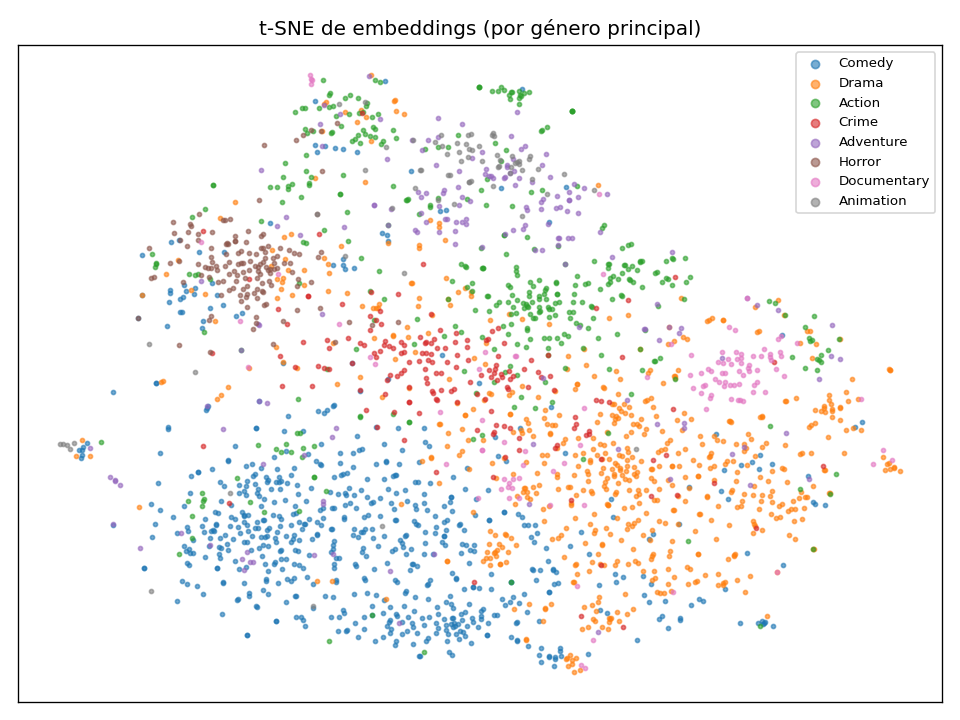
\includegraphics[width=0.74\textwidth]{fase4_tsne_embeddings.png}
\caption{Proyección t-SNE de los \textit{embeddings} de película aprendidos, coloreados por género principal. La estructura por géneros emerge \textbf{sin} que el modelo haya visto los géneros: evidencia de que el espacio latente es semánticamente significativo.}
\label{fig:tsne}
\end{figure}

% --------------------------------------------------------- NeuMF
\subsection{NeuMF — Neural Collaborative Filtering}
\begin{modelcard}{NeuMF (GMF $\oplus$ MLP) \hfill \noserv}
\textbf{Qué es.} La arquitectura \textit{Neural Collaborative Filtering} canónica: una rama \textbf{GMF} (producto elemento a elemento) y una rama \textbf{MLP} (no lineal) fusionadas, con sesgos.\\[3pt]
\textbf{Cómo funciona.} Dos juegos de \textit{embeddings} (GMF y MLP), MLP con capas \code{64-32-16} + \textit{dropout}, fusión y cabeza lineal; misma salida acotada y \textit{early stopping}.\\[3pt]
\textbf{Por qué (NO se sirve).} Iguala al SVD pero \textbf{no supera} al MF+Bias en este volumen, y su brazo MLP hace que el vector de usuario sea no lineal $\Rightarrow$ \textbf{no admite \textit{folding-in} barato} para usuarios nuevos. Queda entrenado y versionado como comparación.\\[3pt]
\textbf{Para qué / Dónde.} \emph{Documentación:} notebook 04, etapa \code{train\_dl}. \emph{Web-app:} no se sirve.\\[3pt]
\textbf{Métricas (test, nb04).} RMSE 0,8196 · MAE 0,6208 ($\sim$2,8\,M parámetros, vs 1,4\,M del MF+Bias).
\end{modelcard}

% --------------------------------------------------------- Encoder
\subsection{Encoder semántico — Sentence-Transformers (MiniLM)}
\begin{modelcard}{Encoder \texttt{paraphrase-multilingual-MiniLM-L12-v2} \hfill \enprod}
\textbf{Qué es.} Modelo \textit{transformer} preentrenado (inferencia, CPU) que convierte texto en \textit{embeddings} densos. Multilingüe: permite consultas en español sobre descriptores en inglés.\\[3pt]
\textbf{Cómo funciona.} Codifica un \textbf{descriptor} por película (título + géneros + \textit{top} 12 \textit{tags} genome con relevancia $\geq 0{,}5$) en un vector L2-normalizado.\\[3pt]
\textbf{Por qué.} Habilita búsqueda por \textbf{significado} (no por coincidencia de texto), en lenguaje natural y multilingüe, sin entrenar nada.\\[3pt]
\textbf{Para qué / Dónde.} \emph{Documentación:} notebook 05, etapa \code{index} del pipeline. \emph{Web-app:} página \textbf{Buscar}. \emph{Backend:} \code{ml/semantic.py}; artefacto \code{models/rag\_index/}.
\end{modelcard}

% --------------------------------------------------------- FAISS
\subsection{FAISS — Índice vectorial}
\begin{modelcard}{FAISS (inner product = coseno) \hfill \enprod}
\textbf{Qué es / Cómo funciona.} Índice de búsqueda de vecinos sobre los vectores normalizados del encoder; producto interno equivalente a similitud coseno. Un \textit{re-ranking} mezcla la similitud semántica con un \textit{prior} de popularidad ($\alpha=0{,}25$).\\[3pt]
\textbf{Por qué / Para qué.} Recuperación rápida de candidatos relevantes a la consulta; el \textit{re-ranking} equilibra relevancia y calidad.\\[3pt]
\textbf{Dónde.} \emph{Documentación:} notebook 05, etapa \code{index}. \emph{Web-app:} página \textbf{Buscar}. \emph{Backend:} \code{ml/semantic.py}.
\end{modelcard}

% --------------------------------------------------------- RAG LLM
\subsection{Capa generativa RAG — Claude (LLM)}
\begin{modelcard}{RAG generativo (\texttt{claude-haiku-4-5}) \hfill \enprod}
\textbf{Qué es.} \textit{Retrieve--Augment--Generate}: recupera películas relevantes con FAISS y redacta una recomendación en lenguaje natural con un LLM.\\[3pt]
\textbf{Cómo funciona.} El contexto recuperado se inyecta en un \textit{prompt}; la generación es opcional (\code{generate=true}) y degrada a una plantilla si no hay API key.\\[3pt]
\textbf{Por qué / Para qué.} Convierte la búsqueda en una experiencia \textbf{conversacional}.\\[3pt]
\textbf{Dónde.} \emph{Documentación:} notebook 05. \emph{Web-app:} \textbf{Buscar} con respuesta generada. \emph{Backend:} \code{src/generate.py}, expuesto en \code{/api/search/semantic?generate=true}.
\end{modelcard}

% ============================================================================
\section{Comparativas y resultados reales}
\label{sec:comparativas}

\subsection{Fase 3 — Modelos clásicos (\textit{test} temporal warm-start)}
\begin{center}
\small
\begin{tabularx}{\textwidth}{@{}X r r c@{}}
\toprule
\textbf{Modelo} & \textbf{RMSE} $\downarrow$ & \textbf{MAE} $\downarrow$ & \textbf{Estado} \\
\midrule
\textbf{SVD} (campeón) & \textbf{0,865} & \textbf{0,656} & \enprod \\
KNN-Baseline (item) & 0,893 & 0,669 & \noserv \\
AutoML $\rightarrow$ BaselineOnly & 0,923 & 0,704 & \proceso \\
NMF & 0,936 & 0,713 & \noserv \\
Baseline (Pop. bayesiana) & 1,009 & 0,792 & \enprod \\
\bottomrule
\end{tabularx}
\end{center}

\subsection{Fase 4 — Deep Learning vs clásico (mismo \textit{split} 70/15/15)}
\begin{center}
\small
\begin{tabularx}{\textwidth}{@{}X l r r@{}}
\toprule
\textbf{Modelo} & \textbf{Familia} & \textbf{Test RMSE} $\downarrow$ & \textbf{Test MAE} $\downarrow$ \\
\midrule
\textbf{MF+Bias (DL)} & Deep Learning & \textbf{0,8046} & \textbf{0,6113} \\
SVD (clásico, mismo \textit{split}) & Factorización & 0,8194 & 0,6212 \\
NeuMF (DL) & Deep Learning & 0,8196 & 0,6208 \\
\bottomrule
\end{tabularx}
\end{center}

\begin{infobox}[Rigor metodológico]
Las dos tablas usan \textbf{protocolos de evaluación distintos} (la Fase 3 usa un \textit{split} temporal warm-start; la Fase 4 un \textit{split} 70/15/15 sobre \code{ratings\_knn\_10pct}), por lo que sus RMSE \textbf{no son comparables entre fases}. La conclusión clave de la Fase 4 es que, en una comparación \emph{justa} (mismo \textit{split}, sesgos, salida acotada), \textbf{el Deep Learning iguala o supera al clásico}; la diferencia que se atribuía antes a ``superioridad del SVD'' era un artefacto de comparar datasets distintos.
\end{infobox}

% ============================================================================
\section{Qué se usa en producción y dónde}
\label{sec:produccion}
El sistema combina los modelos según el contexto, ubicando cada uno donde su fortaleza no choca con el \textit{cold-start}.

\begin{center}
\footnotesize
\begin{tabularx}{\textwidth}{@{}L{2.7cm} L{2.6cm} L{3.0cm} X@{}}
\toprule
\textbf{Modelo} & \textbf{Artefacto} & \textbf{Endpoint} & \textbf{Página web / Por qué} \\
\midrule
Pop. bayesiana & \code{baseline\_scores.pkl} & \code{/recommendations/*} & Invitados / \textit{cold-start}. \\
SVD + \textit{folding-in} & \code{svd\_model.pkl} & \code{/recommendations/home}, \code{/affinity} & \textbf{Para Ti}, afinidad: personalización ligera. \\
KMeans personas & (en \code{svd\_model.pkl}) & \code{/meta/personas} & \textbf{Perfil}: comunidad del usuario. \\
\textbf{MF+Bias (DL)} & \code{dl\_item\_embeddings.pkl} & \code{/movies/\{id\}/similar?method=dl} & \textbf{Ficha}: ``películas similares'' (sin \textit{cold-start}). \\
Encoder + FAISS & \code{rag\_index/} & \code{/search/semantic} & \textbf{Buscar}: lenguaje natural. \\
RAG (Claude) & --- (API) & \code{/search/semantic?generate=true} & \textbf{Buscar}: respuesta redactada. \\
\bottomrule
\end{tabularx}
\end{center}

\begin{infobox}[Diseño defensivo]
La similitud DL tiene \textbf{\textit{fallback} transparente}: si \code{dl\_item\_embeddings.pkl} no existe o una película no fue modelada, \code{engine.similar\_dl()} cae al espacio latente del SVD sin romper nada. La capa generativa degrada a plantilla sin API key. El sistema nunca falla por un artefacto ausente.
\end{infobox}

% ============================================================================
\section{MLOps: cómo funciona}
\label{sec:mlops}
La capa MLOps (CRISP-DM Fase 4) hace que el ciclo de vida de los modelos sea \textbf{reproducible, versionado, trazable y monitoreado}. Se apoya en seis pilares.

\subsection{1. Pipeline reproducible y orquestado}
\code{src/pipeline.py} encadena \textbf{etapas idempotentes} dirigidas por configuración (semilla fija = 42):
\begin{center}
\code{prepare $\rightarrow$ train $\rightarrow$ train\_dl $\rightarrow$ baseline $\rightarrow$ index $\rightarrow$ evaluate $\rightarrow$ register $\rightarrow$ monitor}
\end{center}
\begin{lstlisting}[language=bash]
python -m src.pipeline all        # ciclo completo
python -m src.pipeline train_dl   # solo Deep Learning
make pipeline                     # equivalente dentro de Docker
\end{lstlisting}

\subsection{2. Configuración como código}
Nada de números mágicos: todo vive en \code{config/*.yaml}.
\begin{itemize}
\item \code{pipeline.yaml} — rutas, hiperparámetros de SVD y \code{deep\_learning}, protocolo de evaluación, MLflow.
\item \code{rag.yaml} — encoder, índice FAISS, \textit{re-ranking}, capa generativa.
\item \code{monitoring.yaml} — umbrales de alerta y política de reentrenamiento.
\end{itemize}

\subsection{3. Tracking de experimentos (MLflow)}
Cada ejecución de \code{train\_dl} y \code{evaluate} abre un \textit{run} de MLflow que registra parámetros, métricas y \textit{tags}. \textbf{Verificado} en Docker: el experimento \code{omnirec-fase4-mlops-rag} contiene los \textit{runs} \code{train\_dl} (con \code{mf\_bias\_test\_rmse=0.8046}, \code{neumf\_test\_rmse=0.8191}, parámetros y tiempos) y \code{evaluate}. Degrada a \textit{no-op} si MLflow no está, sin romper el pipeline.

\subsection{4. Registro y versionado de artefactos (SHA256)}
\code{src/registry.py} versiona cada artefacto en \code{models/registry/<nombre>/<versión>/} con un \textbf{manifiesto SHA256} (integridad y trazabilidad), \code{dataset\_version}, métricas y linaje (\code{parent}). El alias \code{current.json} apunta a la versión en producción, habilitando \textbf{promoción y \textit{rollback}}. \textbf{Verificado} (pipeline completo en Docker): cuatro artefactos versionados.
\begin{center}
\footnotesize
\begin{tabularx}{\textwidth}{@{}l l X@{}}
\toprule
\textbf{Artefacto} & \textbf{Versión \textit{current}} & \textbf{Métricas en el manifiesto} \\
\midrule
\code{svd\_model} & \code{2026.06.24-1} & recomendador (RMSE, NDCG\@10). \\
\code{baseline\_scores} & \code{2026.06.24-1} & estrategia bayesiana. \\
\code{rag\_index} & \code{2026.06.24-1} & recuperación (P\@k, cobertura). \\
\code{dl\_embeddings} & \code{2026.06.24-1} & Test RMSE 0,8046, MAE 0,6113, linaje. \\
\bottomrule
\end{tabularx}
\end{center}

\subsection{5. Evaluación con protocolo definido}
\code{src/evaluate.py} mide el recomendador (\code{rmse}, \code{mae}, \code{hitrate@10}, \code{ndcg@10}, vía \textit{folding-in}) y la recuperación (\code{mean\_precision@k}, \code{coverage\_genome}). \textbf{Verificado} en Docker: \code{rmse=0.8823}, \code{ndcg@10=0.2488}, \code{P@k=0.8833}, cobertura $0{,}25$.

\subsection{6. Monitoreo, \textit{drift} y política de reentrenamiento}
\code{src/monitor.py} genera un reporte JSON que combina calidad, \textit{drift} y degradación, y dispara alertas contra \code{monitoring.yaml}:
\begin{center}
\footnotesize
\begin{tabularx}{\textwidth}{@{}X l@{}}
\toprule
\textbf{Señal monitoreada} & \textbf{Umbral} \\
\midrule
Caída de NDCG\@10 vs versión \code{current} (SVD) & $>5\%$ \\
Subida de Test RMSE del modelo DL vs \code{current} & $>5\%$ \\
\textit{Drift} de la distribución de \textit{ratings} (PSI antiguo vs reciente) & $>0{,}2$ \\
Cobertura del recomendador / genome & $<0{,}6$ \\
Frescura de datos (días desde el último \textit{rating}) & $>30$ \\
\bottomrule
\end{tabularx}
\end{center}
La \textbf{política de reentrenamiento} (disparadores) considera 50\,000 \textit{ratings} nuevos acumulados, un \textit{schedule} mensual de respaldo y un \textbf{\textit{guardrail}}: solo promueve a \code{current} si las métricas no empeoran. \textbf{Verificado}: el reporte incluye el bloque \code{deep\_learning} (con \code{rmse\_rise\_pct\_vs\_current}) y detectó correctamente 3 alertas reales del dataset estático (\textit{drift} de \textit{ratings}, cobertura genome y antigüedad de datos).

\subsection{Despliegue reproducible (Docker)}
El \code{docker-entrypoint.sh} construye artefactos de forma \textbf{idempotente} en el primer arranque (índice, SVD, baseline, y ahora el modelo DL vía \code{train\_dl} + \textit{export} + \textit{register}). Las imágenes fijan dependencias con su justificación (p.\,ej. \code{numpy<2} por scikit-surprise, \code{torch==2.4} por estabilidad). Backend, MLflow y Jupyter comparten la misma imagen (paridad de entorno).

\begin{infobox}[Cobertura MLOps por modelo]
Los cuatro artefactos de servicio (SVD, baseline bayesiano, \textit{embeddings} DL, índice RAG) están \textbf{en el pipeline}, \textbf{trackeados en MLflow} y \textbf{versionados} con manifiestos SHA256. El modelo Deep Learning quedó completamente integrado al ciclo MLOps, reproducible en los tres entornos (notebook, local y Docker) con el mismo Test RMSE \textbf{0,8046}.
\end{infobox}

% ============================================================================
\section{La plataforma web (OmniCine)}
\label{sec:webapp}
El frontend Next.js consume la API REST de FastAPI. El recorrido del usuario activa distintos modelos:

\begin{center}
\footnotesize
\begin{tabularx}{\textwidth}{@{}l X l@{}}
\toprule
\textbf{Página} & \textbf{Función} & \textbf{Modelo(s)} \\
\midrule
\code{/cartelera} & Explorar el catálogo (filtros, orden) & Popularidad / catálogo \\
\code{/buscar} & Búsqueda en lenguaje natural & Encoder + FAISS + RAG \\
\code{/para-ti} & Recomendaciones personalizadas & SVD + \textit{folding-in} / baseline \\
\code{/pelicula/[id]} & Ficha + ``películas similares'' + afinidad & \textbf{MF+Bias (DL)} + SVD \\
\code{/perfil} & ``Tu comunidad'' & KMeans personas \\
\code{/login}, \code{/registro} & Autenticación & --- \\
\bottomrule
\end{tabularx}
\end{center}

\textbf{Flujo invitado $\rightarrow$ usuario.} Los invitados acumulan \textit{feedback} en \code{localStorage}; al iniciar sesión se migra al backend (\code{/ratings/sync}), de modo que las recomendaciones personalizadas (SVD \textit{folding-in}) y la \textit{persona} (KMeans) se activan inmediatamente sobre el historial recién migrado.

% ============================================================================
\section{Reproducibilidad y ejecución}
\label{sec:repro}
\begin{lstlisting}[language=bash]
# Stack completo (backend + web + MLflow)
make up-all                  # web: localhost:3000  |  MLflow: localhost:5001

# Pipeline MLOps de extremo a extremo (dentro del backend)
docker compose run --rm backend python -m src.pipeline all

# Reentrenar y versionar solo el modelo Deep Learning
docker compose run --rm backend python -m src.pipeline train_dl
docker compose run --rm backend python -m src.pipeline register

# Notebooks (Jupyter sobre la misma imagen)
make jupyter                 # http://localhost:8888
\end{lstlisting}

\begin{infobox}[Garantías de reproducibilidad]
Semilla fija (42) en todo el pipeline, dependencias fijadas con su motivo, \textit{splits} deterministas, hashes SHA256 por artefacto y configuración como código. El mismo Test RMSE (0,8046) se obtiene en notebook, en local y en Docker.
\end{infobox}

% ============================================================================
\section{Conclusiones}
\label{sec:conclusiones}
\begin{itemize}
\item El sistema integra \textbf{tres familias de modelos} (factorización clásica, redes neuronales de \textit{embeddings} y recuperación semántica con \textit{transformers} + LLM), ubicando cada una donde su fortaleza es máxima y el \textit{cold-start} no la penaliza.
\item En una comparación \textbf{justa}, el Deep Learning (MF+Bias) \textbf{iguala o supera} al clásico (RMSE 0,8046 vs 0,8194), y sus \textit{embeddings} capturan estructura semántica real, hoy explotada en ``películas similares''.
\item \textbf{Todo lo que se sirve está en MLOps y versionado}: pipeline reproducible, \textit{tracking} en MLflow, \textit{registry} con manifiestos SHA256 y linaje, y monitoreo de \textit{drift} y degradación, verificado de extremo a extremo en Docker.
\item La web-app \textit{OmniCine} traduce cada modelo en una funcionalidad concreta y comprensible para el usuario final, con \textit{fallbacks} defensivos que garantizan disponibilidad.
\end{itemize}

\vfill
\begin{center}
\footnotesize\color{omnigray}
OmniRec-Movies · Informe Técnico Integral · MovieLens 25M · CRISP-DM · \today
\end{center}

\end{document}
